\section[Strojové učení]{Strojové učení \& Neuronové sítě}

\begin{frame}{Běžné programování vs.\ strojové učení}

    {\large \textbf{Programování řešení}}

    \begin{itemize}

        \item<2-> Jsme schopni problém \textbf{formálně popsat} jasnými koncepty

        \item<3-> Program je jednoznačný \textbf{návod}, jak s koncepty zacházet

    \end{itemize}

    \vspace{10pt}

    \visible<4->{%
    \begin{beamercolorbox}{blockcolor}
    {\color{ufal} Příklad -- E-shop:} {\it Koncepty: zboží, sklad, zákazník,
    objednávka} \\
    \quad Udělat objednávku, odeslat objednávku = jednoduchý algoritmus
    \end{beamercolorbox}}

    \vspace{20pt}

    \visible<5->{{\large \textbf{Učení řešení}}}

    \begin{itemize}

	    \item<6-> Máme \textbf{příklady} vstupů a výstupů a \textbf{metriku} jak dobré je řešení

        \item<7-> Nejsme schopni do důsledku napsat návod, jak úlohu řešit

    \end{itemize}

    \vspace{10pt}

    \visible<8->{%
    \begin{beamercolorbox}[]{blockcolor}
    {\color{ufal} Příklad -- automatický překlad:} {\it neexistuje návod, pro člověka, který nerozumí oběma jazykům} \\
    \quad Existuje mnoho přeložených textů, co se dají použít pro trénování
    \end{beamercolorbox}}

\end{frame}

% ----------------------------------------------------------------------------

\begin{frame}{Obecné schéma}

    \centering
\scalebox{.8}{%
\begin{tikzpicture}%
[   normal arrow/.style={draw,-triangle 45,very thick},
    big box/.style={draw=####1!20!black, fill=####1!60, minimum width=9em, minimum height=9em, rectangle, align=center},
    small box/.style={draw, minimum height=5mm, minimum width=####1, rectangle}
]
\node[big box = RoyalBlue] (d) at (1, -5) {};
\node[above] at (d.north) {};
\node[below, align=center] at (d.north) {data};
\node[big box = ForestGreen] (a) at (7, -5) {};
\node[below, align=center] at (a.north) {učící algoritmus};
\node[big box = Dandelion] (m) at (14, -5) {};
\node[below, align=center] at (m.north) {model};

\path[normal arrow] (d) -- (a);
\path[normal arrow] (a) -- (m);

\foreach \x in {1,...,3} {%
	\node[small box = 5em] (x\x) at (0.4, -3.4 - \x * 0.8) {$x_{\x}$};
	\node[small box = 1.5em] (y\x) at (2.2, -3.4 - \x * 0.8) {$y_{\x}$};
	\path[draw] (x\x) -- (y\x);
}
\node[] (xc) at (0.4, -3.2 - 4 * 0.8) {$\vdots$};
\node[] (yc) at (2.2, -3.2 - 4 * 0.8) {$\vdots$};

\node[small box = 5em] (x) at (14, -2) {$x$};
\node[small box = 1.5em] (y) at (14, -8) {$y$};

\path[normal arrow] (x) -- (m);
\path[normal arrow] (m) -- (y);

\node[small box = 6em] (meta) at (7, -5) {hyperparametry};

\node[small box = 6em] (par-alg) at (14, -5) {parametery};
\node[small box = 6em] (par) at (14, -6) {algoritmus};

\end{tikzpicture}}

    \vspace{1em}

    \visible<2->{Cíl učení = model, který \textbf{generelalizuje} pro nová data.}

\end{frame}

% ----------------------------------------------------------------------------

\begin{frame}{Příklad strojového učení}

    \centering
    \begin{tabular}{lcc}
        & \visible<1->{\bf Rozpoznávání objektů & \bf Strojový překlad} \\ \midrule

        \visible<2->{
        \bf Data & $x$: RGB obrázek           & $x$: Věta ve zrdojovém jazyce \\
             & $y$: Pozice a typ objektu  & $y$: Věta v cílovém jazyce \\ \midrule}

         \visible<3->{
        \bf Učící algoritmus & \multicolumn{2}{c}{Minimalizace chyby, gradient descent} \\ \midrule}

    \visible<4->{
        \bf Model & konvoluční neuronová síť & Transformer (neuronová síť)  \\ \midrule}

    \visible<5->{
    \bf Algoritmus & sliding window přes obrázek & autoregresivní dekódování \\
               & (obdélníky různých velikostí) & (vždy jedno slov na výstup, \\
               &  & jde na vstup v dalším kroku)}

    \end{tabular}


\end{frame}

% ----------------------------------------------------------------------------

\begin{frame}{Generalizace vs. přeučení}

    \begin{center}
    \includegraphics{./img/overfitting.png} \\
    {\tiny Zdroj: https://www.geeksforgeeks.org/underfitting-and-overfitting-in-machine-learning}
    \end{center}

    \visible<2->{
        \textbf{\Large Přeučení} = model si zapamatuje trénovací data, funguje dobře jenom pro data, která vypadají jako trénovací} \\
    \visible<3->{\hfill \Large\bf \ldots nejčastější zdroj chyb a diskriminace}

\end{frame}

% ----------------------------------------------------------------------------

\begin{frame}{Neuronové sítě: Jeden neuron}

    \begin{columns}
        \column{.45\textwidth}
        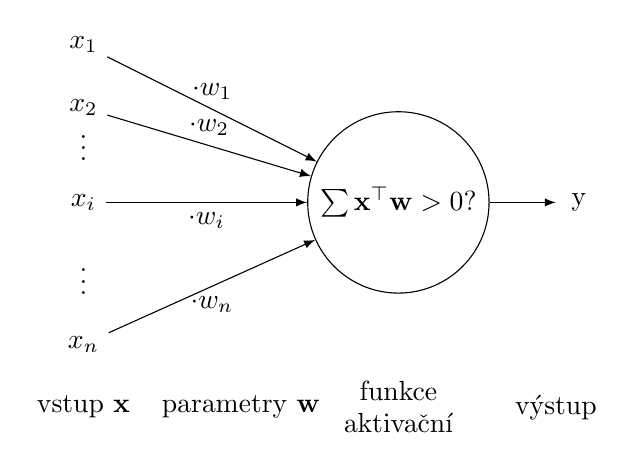
\begin{tikzpicture}[]

\tikzset{>=latex}
\def\inputX{-4.0}
\def\labelY{-2.6}

\draw (0,\labelY - 0.2) node {aktivační};
\draw (0,\labelY + 0.2) node {funkce};

\draw (\inputX,\labelY) node {vstup $\mathbf{x}$};

\draw (\inputX / 2,\labelY) node {parametry $\mathbf{w}$};

\draw (2.0, \labelY) node {výstup};


\draw (0,0) node[draw,circle](neuron) {$\sum \mathbf{x}^\top\mathbf{w} > 0$?};
    \draw[->] (neuron) -- (2,0) node {~~~~~y};

\draw (\inputX,0) node {$x_i$} edge[->] node[anchor=north, pos=.5] {$\cdot w_i$} (neuron);

\draw (\inputX,2.0) node {$x_1$} edge[->]
    node[anchor=south, pos=.5] {$\cdot w_1$} (neuron);
\draw (\inputX,1.2) node {$x_2$} edge[->]
    node[anchor=south, pos=.5] {$\cdot w_2$} (neuron);

\draw (\inputX,0.8) node {$\vdots$};

\draw (\inputX,-0.9) node {$\vdots$};

\draw (\inputX,-1.8) node {$x_n$} edge[->]
    node[anchor=north, pos=.5, below] {$\cdot w_n$} (neuron);

\end{tikzpicture}

        \column{.45\textwidth}

        \begin{itemize}[<+->]

            \item Vstupy = reálná čísla

            \item Smíchají s různými vahami

            \item Začátek v 50.\ letech, inspirace představou o neuronu
                ze 40.\ let

            \item Dnes \textbf{nic společného} s biologickými neurony

        \end{itemize}

    \end{columns}

\end{frame}

% ----------------------------------------------------------------------------

\begin{frame}{Neuronová síť: Více vrstev}

    \centering
    Úloha: rozpoznat písmeno z~mřížky 4$\times$4 pixely

    \vspace{10pt}

    \includegraphics{./img/feedforward.pdf}

\end{frame}

% ----------------------------------------------------------------------------

\begin{frame}{Neuronová síť}

    \begin{columns}
        \column{.4\textwidth}

        \scalebox{.75}{\def\layerA{7}
\def\layerB{9}
\def\layerC{9}
\def\layerD{3}
\def\step{2}
\def\size{3pt}

\begin{tikzpicture}[]


\foreach \i in {0,...,\layerA} {
	\draw (0,-0.25 -0.4 * \i) circle (\size) node(layer_1_\i) {};
}
\draw (0, 0.5) node {\small vstup};

\foreach \i in {0,...,\layerB} {
	\draw (\step,-0.4 * \i) circle (\size) node(layer_2_\i) {};
}

\foreach \i in {0,...,\layerC} {
	\draw (2 * \step,-0.4 * \i) circle (\size) node(layer_3_\i) {};
}

\draw (1.5 * \step, 0.5) node {\small skryté vrstvy};

\foreach \i in {0,...,\layerD} {
	\draw (3 * \step,-1 - 0.4 * \i) circle (\size) node(layer_4_\i) {};
    \draw[->] (layer_4_\i) -- (3 * \step + 0.4, -1 - 0.4 * \i);
}

\draw (3 * \step, 0.5) node {\small výstup};

\foreach \i in {0,...,\layerA} {
	\foreach \j in {0,...,\layerB} {
        \draw[->] (layer_1_\i) -- (layer_2_\j);
    }
}

\foreach \i in {0,...,\layerB} {
	\foreach \j in {0,...,\layerC} {
        \draw[->] (layer_2_\i) -- (layer_3_\j);
    }
}

\foreach \i in {0,...,\layerC} {
	\foreach \j in {0,...,\layerD} {
        \draw[->] (layer_3_\i) -- (layer_4_\j);
    }
}

\end{tikzpicture}
}

        \column{.5\textwidth}
        \begin{itemize}[<+->]

            \item Organizace do vrstev $\Rightarrow$

            \begin{itemize}[<+->]

                \item Na vstup vrstvy $\sim$ vektor

                \item Vážení vstupů $\sim$ maticové násobení

                \item Výstup vrstvy $\sim$ vektor

            \end{itemize}

        \item Většina výpočtů \textbf{maticové násobení} $\Rightarrow$ rychlé počítání
            na GPU

        \item Výstup NN = \textbf{spojitá funkce} vstupů

        \end{itemize}
    \end{columns}

\end{frame}

% ----------------------------------------------------------------------------

\begin{frame}{Chybová funkce \& Trénování}

    \begin{itemize}[<+->]

        \item Trénování = \textbf{minimalizace chyby} na trénovacích datech

        \item Když je chyba \textbf{spojitá funkce}, můžeme spočítat
            \textbf{derivaci chyby} vzhledem k parametrům

        \item Posunout parametry po směru derivace = snížit chybu

    \end{itemize}

\end{frame}

% ----------------------------------------------------------------------------

\begin{frame}{Problematická trénovací data}

    \visible<1->{
    {\Large\textbf{Stahování z internetu}} --- neprezentativní, extrémní názory
    jsou mnohem víc slyšet, není kontrola nad tím, co je v datech
    \\ \hfill {\footnotesize \citep{bender2021dangers}}}

    \vspace{15pt}

    \visible<2->{
    {\Large\textbf{Crowd-sourcing}} --- využívání levné pracovní síly, tzv. gig
    economy -- vznikají prekarizovaná zaměstnání
    \\ \hfill {\footnotesize \citep[kap. 2]{crawford2021atlas}}}

    \vspace{15pt}

    \visible<3->{
    {\Large\textbf{Vytěžování existujících databází}} --- neplacená práce
    uživatelů, neprůhledné využití dat (např. když za služby vyhledavače platíme daty)
    \\ \hfill {\footnotesize \citep{couldry2019costs}}}

\end{frame}

% ----------------------------------------------------------------------------

\begin{frame}{Problémy učení z dat: Overfitting}

    \begin{itemize}

        \item<1-> Optimalizované metriky nepostihnou všechno \\[1ex]
            \visible<2->{
            \quad\begin{minipage}{360pt}
                \it Vyhledávání vhodných kandidátů podle CV: když doporučím
                samé vhodné kandidáty, ani si nevšimnu, že jsem nedoporučil
                jiné vhodné (třeba podle rasy)
            \end{minipage} \\
            \hfill {\tiny \citep{derous2019your,bender2018data}}}

        \item<3-> Stereotypy můžou být pro model efektivní způsob optimalizace \\

            \visible<4->{
                \includegraphics[width=350pt]{img/doctor.png}} \\
            \visible<5->{
                \includegraphics[width=350pt]{img/sexy_doctor.png} \\
            \hfill {\tiny Příklad \citet[obr.\ 6 a 7]{rozhledy}} }

    \end{itemize}

\end{frame}